\chapter{Liste}

\section{Rappresentazione di una lista attraverso un vettore (matrice)}

{La lista è doppiamente concatenata, ovvero contiene riferimento sia all'elemento precedente che a quello successivo.}

{La costante NULL viene rappresentata da un indice che non appartiene all'insieme degli indici del vettore (0 in pseudocodice, -1 in $C$)}

\begin{figure}[H]
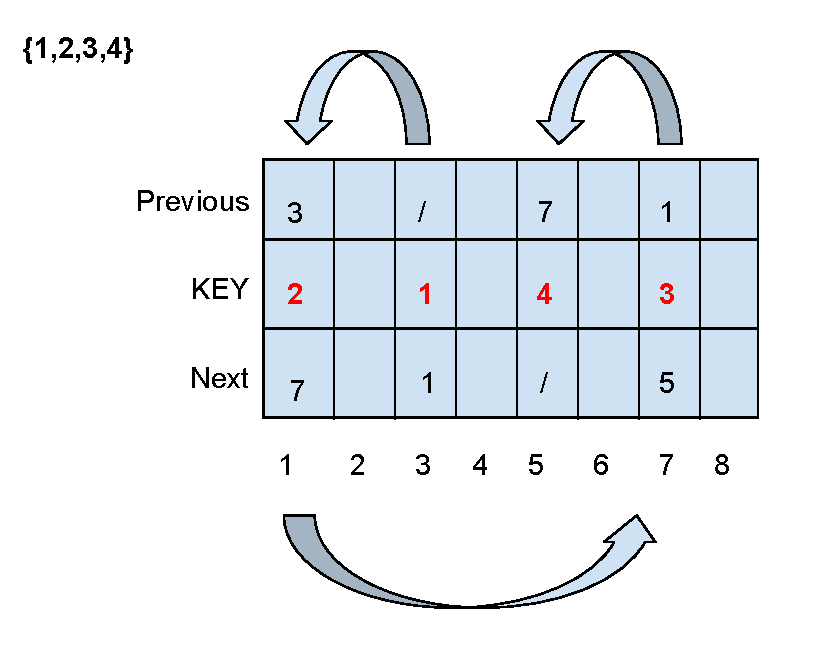
\includegraphics{graphs/lista_matrice.pdf}
\end{figure}

{Analogamente si può creare una lista singolarmente concatenata chiamata FreeList contenente le celle libere (i campi Key e Previous si possono ignorare). Essa verrà utilizzata per l'allocazione di una nuova lista. FreeList è una variabile globale.}

{All'inizio {[}\ldots{}{]} la FreeList contiene TUTTI gli oggetti non allocati.}

{Allocate\_Object()~~~~~~~~~~~~~~~~~~~~~~~~~~~~~~~~}{Complessità $\Theta(1)$}

\lstinputlisting{code/allocate_object.txt}

{\#Inserisce la cella da liberare in testa alla FreeList}

{Free\_Object(x)}{~~~~~~~~~~~~~~~~~~~~~~~~~~~~~~~~Complessità $\Theta(1)$}

\lstinputlisting{code/free_object.txt}
